% ===Lesson 7: Including Graphics and positioning
\documentclass{article}
\usepackage[T1]{fontenc}
\usepackage[margin=1in]{geometry}
\usepackage{verbatim}

% This package allows the use of external graphics
\usepackage{graphicx}

\begin{document}
This lesson shows how you can include external graphics files into your document, how to change their appearance, and how to position or float them automatically.
\vspace{0.5cm}

This is an image of Paul McCartney.

\begin{center}
    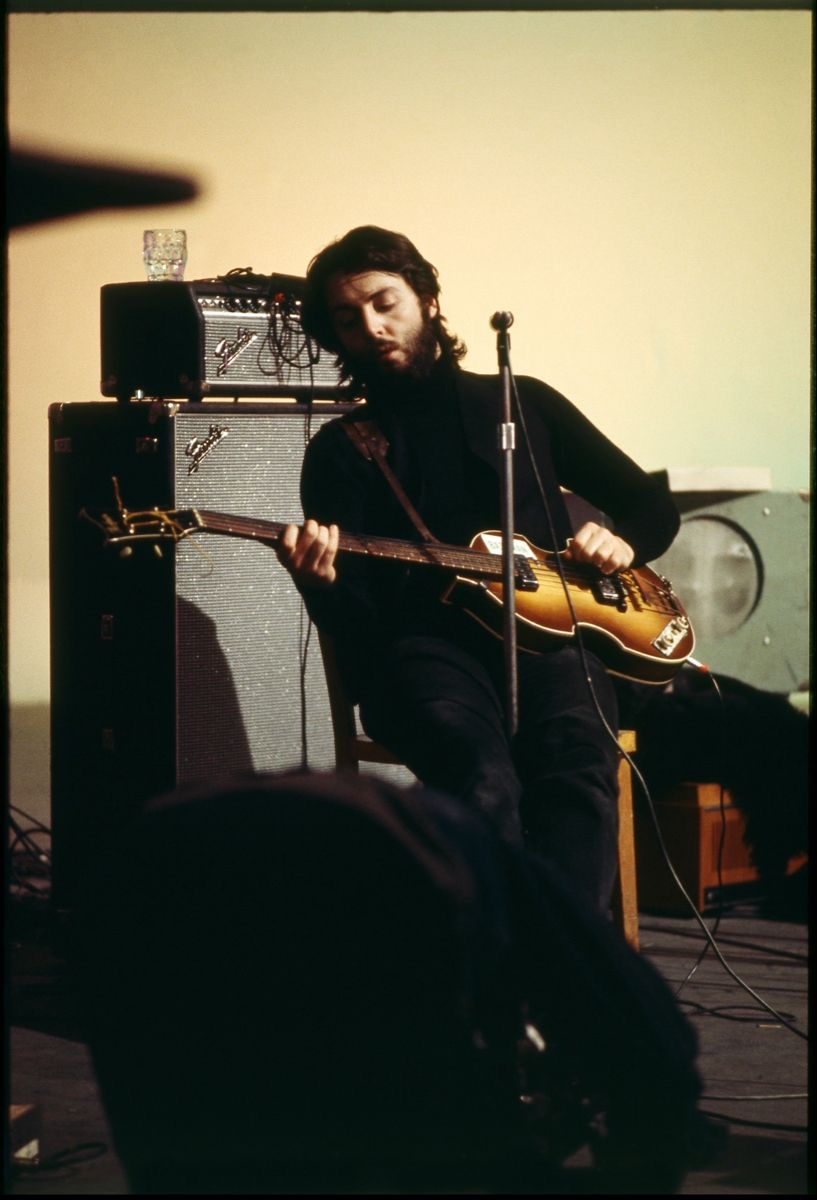
\includegraphics[height=5cm]{image/macca.jpg}
\end{center}

You’ll notice we’ve used a new environment here, \texttt{center}, to place the image horizontally centered on the page. A bit later, we’ll talk more about spacing and positioning.

\begin{verbatim}
    \begin{center}
        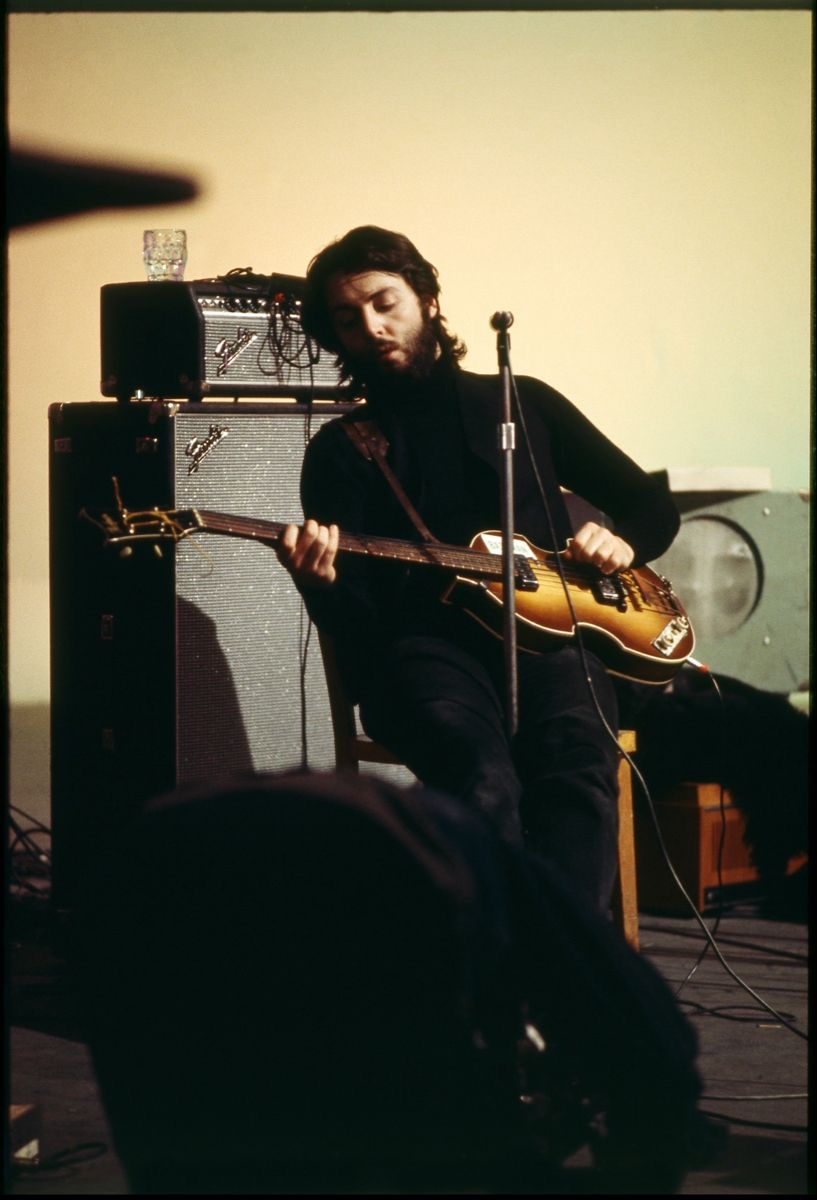
\includegraphics[height=5cm]{image/macca.JPG}
    \end{center}
\end{verbatim}

\section{Altering graphic appearance}
The \texttt{includegraphics} command has many options to control the size and shape of the included images and to trim down material. Some of these are used a lot, so they are worth being aware of.

The most obvious thing to set is the width or the height of an image, which are often given relative to the \texttt{textwidth} or \texttt{linewidth} and \texttt{textheight}. The difference between \texttt{textwidth} and \texttt{linewidth} is subtle and often the result is the same. 

\begin{itemize}
    \item \texttt{textwidth} is the distance from the leftmost to rightmost allowed character on the physical page.
    \item \texttt{textheight} is the distance from the upmost to bottommost allowed character on the physical page.
    \item \texttt{linewidth} is the width of one column of texts.
\end{itemize}

You can also scale images, or rotate them by an angle. The other thing you might want to do is to \texttt{clip} and \texttt{trim} an image.

\begin{verbatim}
    \begin{center}
      \includegraphics[clip, trim = 0 0 50 50]{example-image}
    \end{center}
\end{verbatim}

\section{Making images float}

Example:

\begin{verbatim}
    \documentclass{article}
    \usepackage[T1]{fontenc}
    \usepackage{graphicx}
    \usepackage{lipsum}  % produce dummy text as filler
    
    \begin{document}
    \lipsum[1-4] % Just a few filler paragraphs
    
    Test location.
    \begin{figure}[ht]
      \centering
      \includegraphics[width=0.5\textwidth]{example-image-a.png}
      \caption{An example image}
    \end{figure}
    
    \lipsum[6-10] % Just a few filler paragraphs
    \end{document}
\end{verbatim}

Here LaTeX moves the graphic and the caption away from the Test location text to the top of the second page, because there isn’t room for it on the bottom of the first page. The \texttt{ht} influences where LaTeX can place the float; these two letters mean that it can go where it is in the source (next to Test location) or to the top of a page. You can use up to four position specifiers

\begin{itemize}
    \item\texttt{h}: ‘Here’ (if possible)
    \item\texttt{t}: Top of the page
    \item\texttt{b}: Bottom of the page
    \item\texttt{p}: A dedicated page only for floats
\end{itemize}

You’ll probably spot that we’ve centered the image here using \texttt{centering} rather than the center environment. Inside a float, you should use \texttt{centering} if you want to horizontally center content; this avoids both the float and center environment adding extra vertical space.
\end{document}
% End Lesson 7 (Nov 1 2024)===